\chapter{DNS Rebinding}

DNS rebinding is a computer attack, by which an attacker subverts the
same-origin policy of browsers, this can effectively convert the browser into
an open network proxy \cite{jackson2009protecting}.

\vspace{0.5cm}

\begin{figure}[H]
\begin{center}
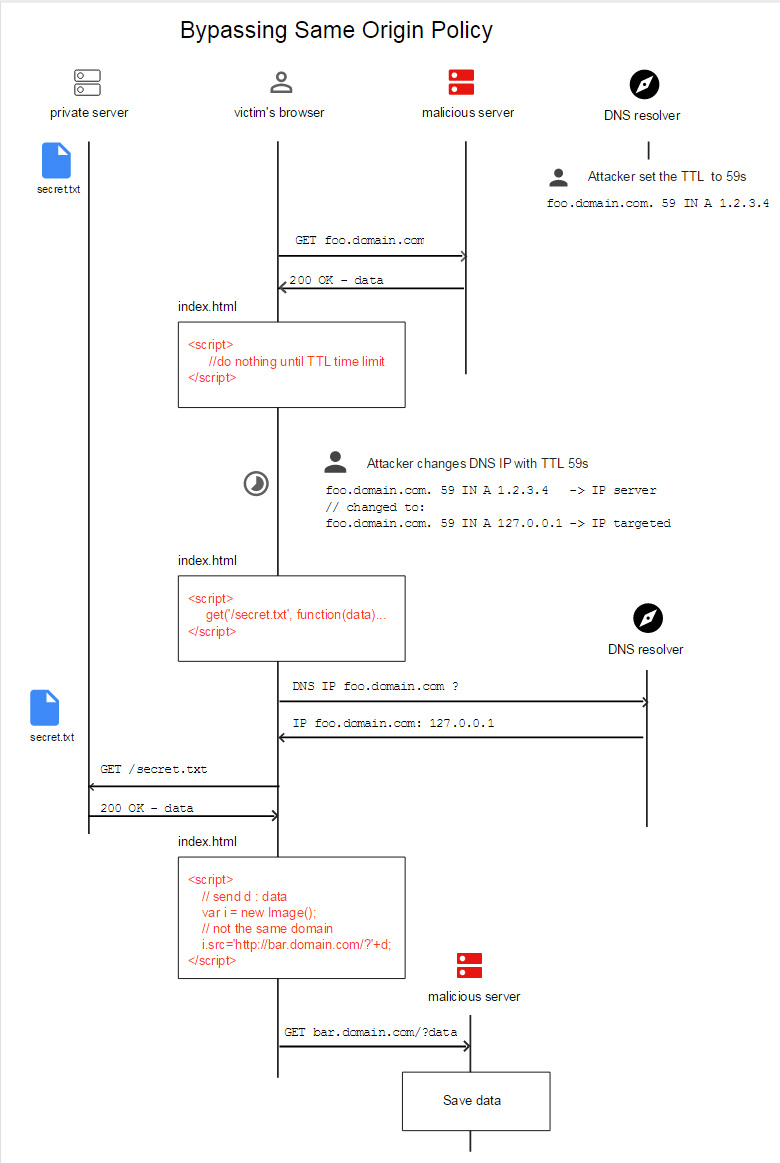
\includegraphics[width=0.59\textwidth,keepaspectratio]
{img/dnsrebindingflow.jpg}
	\caption{DNS Rebinding Flow Diagram (Taken from \cite{vulnsec})}
\end{center}
\end{figure}

\vspace{0.5cm}

DNS Rebinding works by alternating DNS responses between the attacker server IP
and the target machine IP.

For example, an attacker could register a domain name
\texttt{rebind.attacker.com} and set up the DNS responses to alternate between
the legitimate server (e.g. \texttt{10.0.1.55}) and the target server (e.g.
\texttt{127.0.0.1}).

When a user attempts to connect to \texttt{rebind.attacker.com}, assuming the
DNS currently resolves to the attacker server (\texttt{10.0.1.55}), the
attacker can serve specially crafted JavaScript that continually make HTTP
requests waiting for the DNS to resolve to the target IP (\texttt{127.0.0.1}).
At this point the attacker script can make arbitrary HTTP requests which appear
to originate from \texttt{127.0.0.1} effectively bypassing the SOP.

If an application relies on the SOP only for security, and does not explicitly
check Host headers, this can constitute to a security vulnerability. Our
implementation attacks a (now-patched) vulnerable version on the popular
Transmission \cite{transmission} torrent client, which leads arbitrary code
execution (See \S\ref{implementation} for details).
 
\section{Types of DNS Rebinding}

\subsection{Multiple A Records}

\subsection{Time-Varying DNS}

\section{Motives}
